\section{Methods Not Pursued}\label{sec:design_unused_methods}

The below section details methods that were considered or attempted, but ultimately not pursued. We leave this section here as both as advice to future researchers on what methods to try, and as a warning on what to avoid.

\subsection{Road trip}

Before the \caida and \ripe Atlas data was uncovered, an idea for gathering everywhere-to-everywhere data was conceived: take an enormous road trip across the \us, collecting data all along the way. The idea is simple enough in theory and in practice. Just assemble a list of destinations and run constant traceroutes against them on the journey, mapping them to \gps coordinates along the way.

By the end of the trip there would be traceroutes from every point along the route to all the different destinations in the list, many times over. This would yield a significant amount of data. With two people in one car taking shifts in driving (or alternately, staying in hotels for 7-8 hours at a time), it was estimated that the entire US could be roughly circumnavigated in about 7 days.

Fortunately the \caida and \ripe Atlas data sets were discovered well before any serious planning was underway. The idea was immediately nixed, since it turns out that nobody actually wants to spend a week in a car.

\subsection{Network Time Protocol}

\ntp is a protocol designed to synchronize computer clocks around the world. Per the specification for the third version, \ntp is designed to "maintain accuracy and robustness" despite being implemented on "unreliable" networks with "dispersive delays" \cite{rfc1305}. As part of this protocol, the delay, or delta, between the client and server is calculated \cite{rfc5905}. Given the precise nature of this protocol, it would be ideal for this project, which is focused on measuring the network time between geographic locations. The only requirements would be a geographically diverse set of \ntp servers willing to provide the calculated delay values to their peers. Luckily, both parts of this requirement are met -- mostly.

The \ntp specification details a server "mode 6", that allows for "remote control queries", providing a way for remote management of certain aspects of the server \cite{Haberman2019Control4}. One of the these queries, the \texttt{peers} command, prompts the server to return a list of its peers, \footnote{Peers are other \ntp servers that a given server is configured use for synchronization.} along with calculated statistics for these peers -- including the delay. \autoref{fig:sample_ntpq} is an example of such a command using the \texttt{ntpq} tool (with some fields removed for formatting).

\begin{figure}[h]
    \centering
    \begin{minipage}{0.75\textwidth}
    \begin{minted}{text}
>ntpq -c peers 127.0.0.1
     remote           refid      delay   offset  jitter
=======================================================
*ntp1.wpi.edu    130.215.32.36   0.851   -0.076   0.134
+ntp2.wpi.edu    130.215.32.36   0.646   -0.366   0.182
+ntp3.wpi.edu    130.215.144.33  1.376    0.711   0.261
    \end{minted}
    \end{minipage}
    \caption{Sample NTP Mode 6 \texttt{peers} command output}
    \label{fig:sample_ntpq}
\end{figure}

As the example shows, the \texttt{peers} command response includes both delay and jitter calculations for each peer. Coupled with \ip geolocation, requesting the peers from a list of mode 6 \ntp servers would be a straightforward way of getting point to point measurements. And there is no shortage of \ntp servers with mode 6 enabled in the \us: according to the ShadowServer Foundation, which conducts period scans for such servers, as of January 22nd, 2020 there are 522,415 such servers in the country \cite{TheShadowserverFoundationNTPProject}. Additionally, as \cref{fig:ntp_mode_6_us_map} shows, they are distributed across most of the country.

\begin{figure}[h]
    \centering
    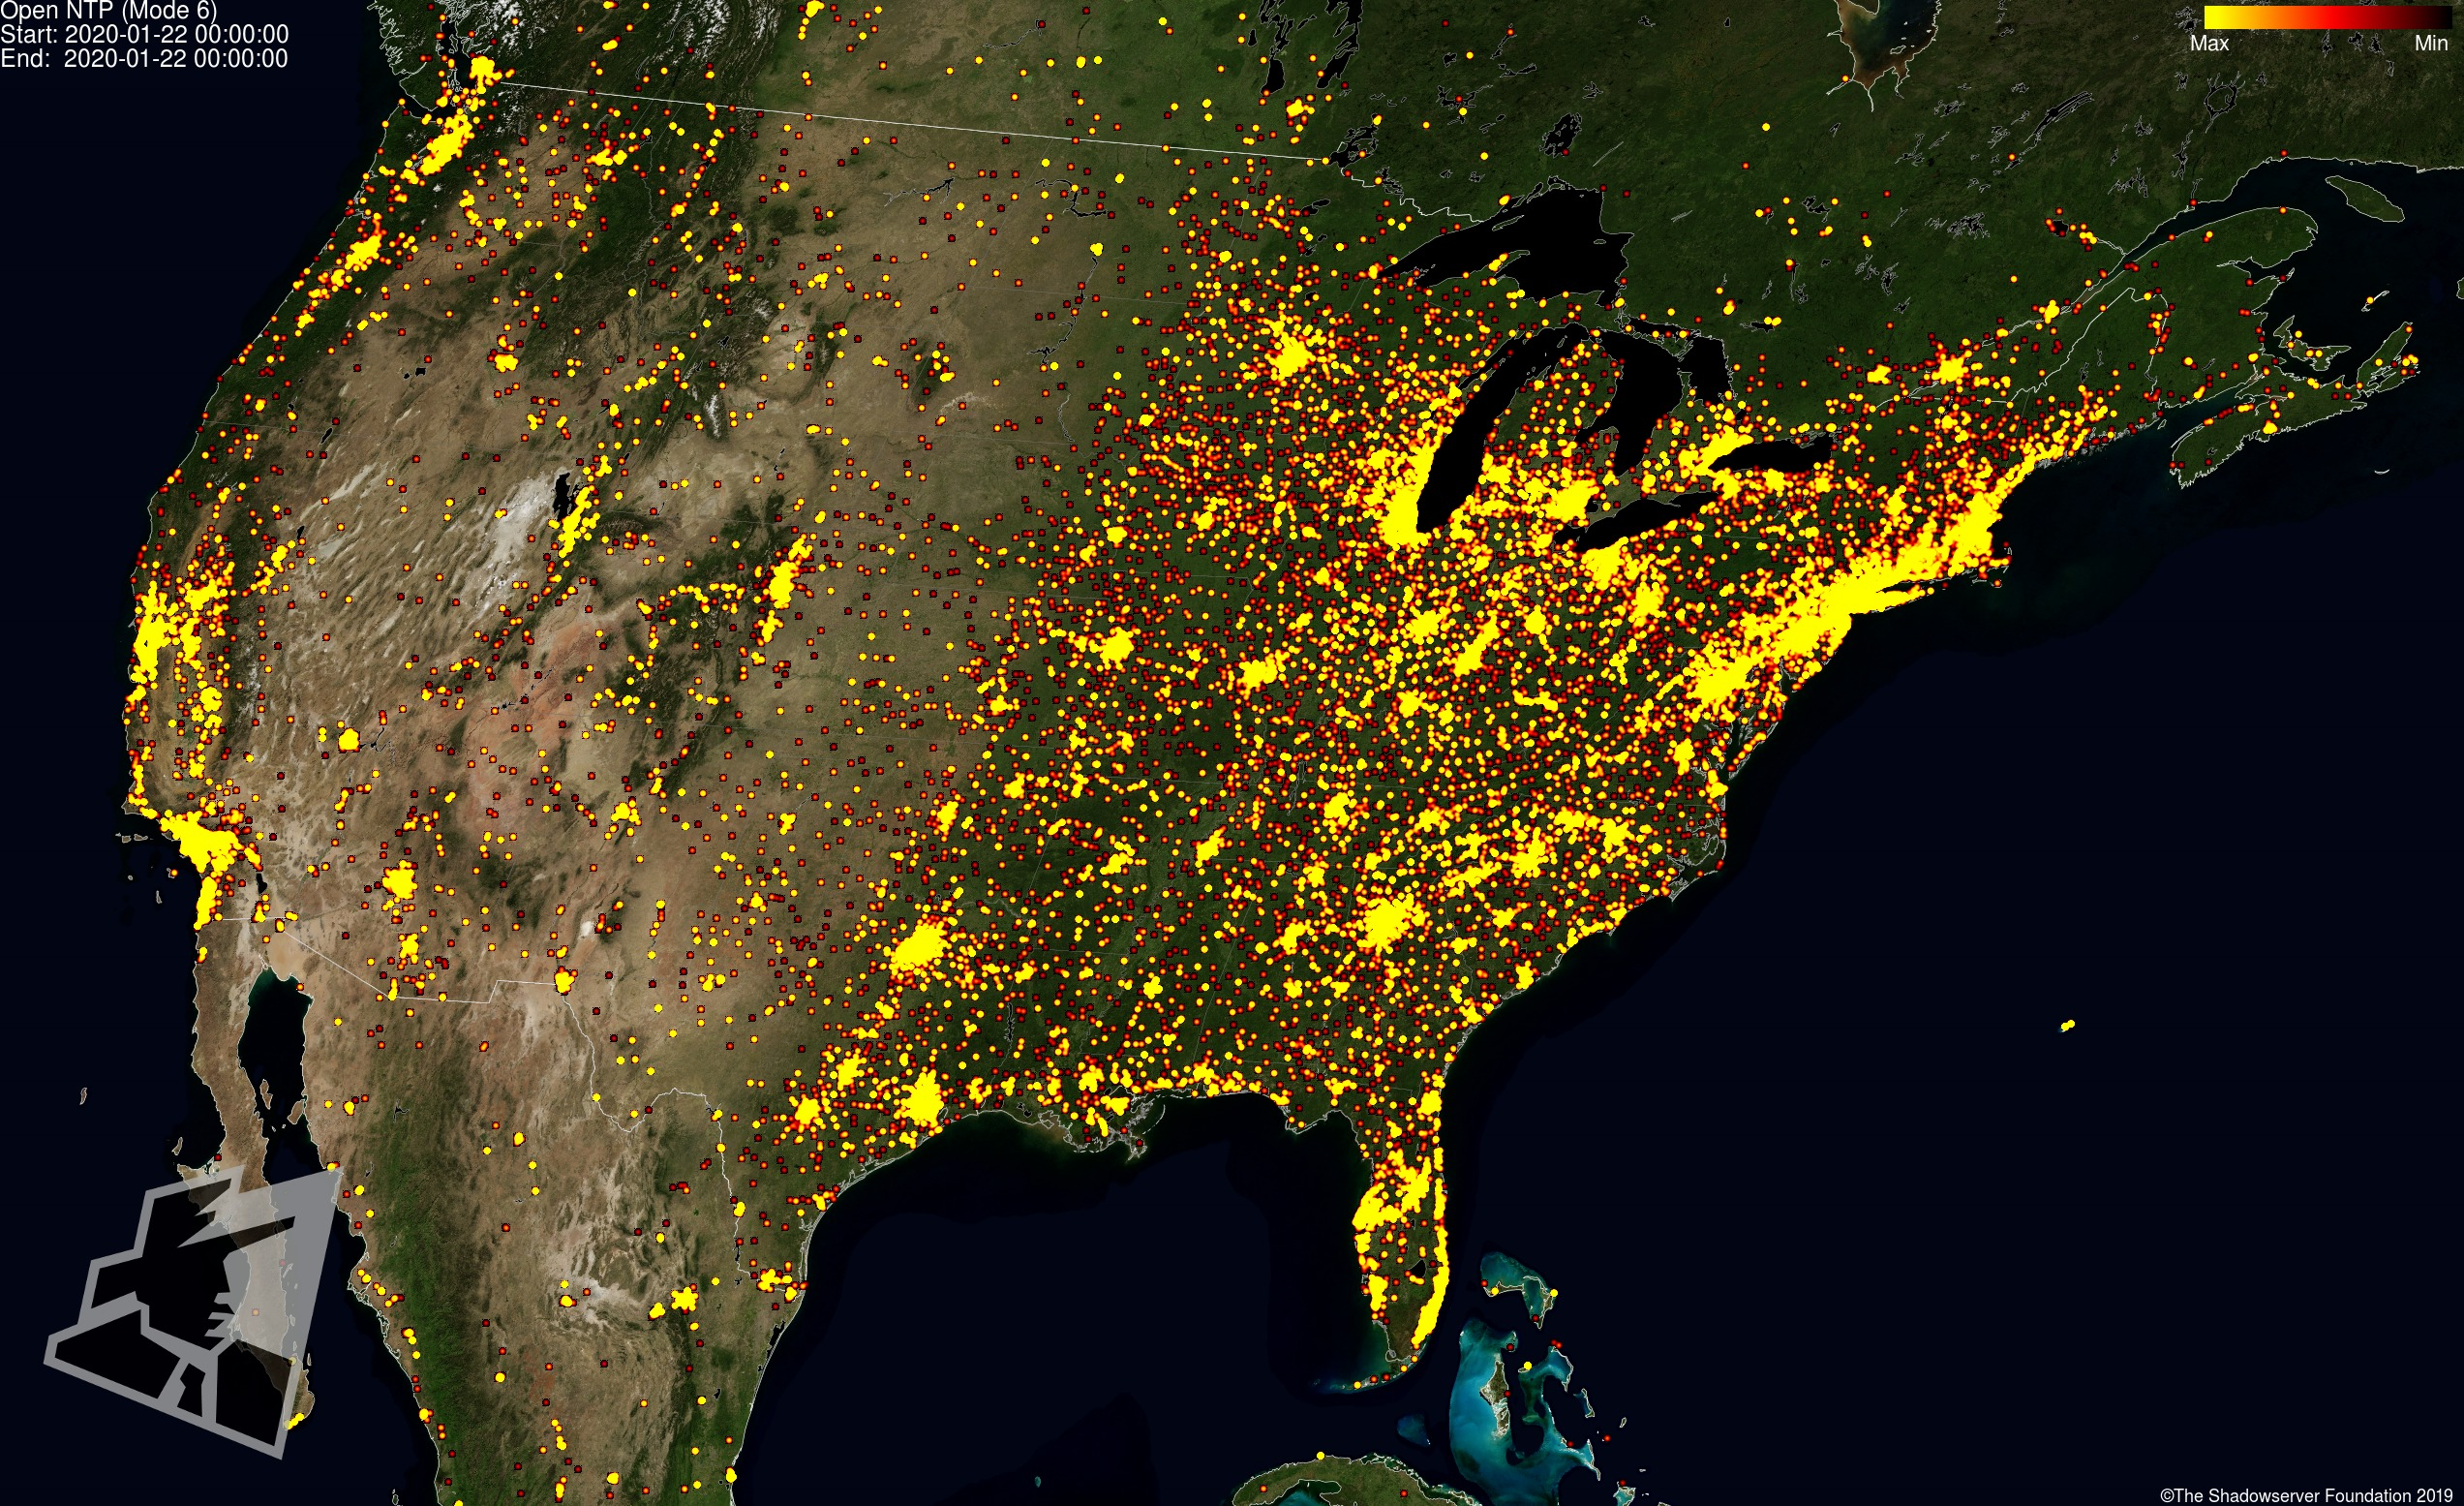
\includegraphics{images/ntpversion_united_states_current.jpg}
    \caption{Distribution of NTP Mode 6 Servers in the US \cite{TheShadowserverFoundationNTPProject}}
    \label{fig:ntp_mode_6_us_map}
\end{figure}

In theory, using these servers and conducting a simple survey of the delay times to each of their peers would be an ideal method for this project. Unfortunately, one of the commands included in mode 6 makes the servers vulnerable to being exploited for use in amplified \ddos attacks \cite{USDepartmentofHomelandSecurity2014NTPCVE-2013-5211}. Thus, despite performing frequent scans for mode 6 servers, the ShadowServer Foundation does not publish a list of such servers, since doing so would pose a security risk. We found no other source of potential servers and proceeded to attempt our own scan of potential \ip address ranges. While we found some potential servers, many lacked any peers and the search was time intensive. Future work may include this method, provided a list of potential servers is available or more time can be dedicated to scanning for them.

\subsection{ISP Mapping}
% FCC fixed broadband deployment map
The \FCC maintains a data set of broadband internet deployment across the \us \cite{FederalCommunicationsCommission}. The data set is composed of a list of census blocks, and contains all of the providers that are within the census block, as well as the maximum, minimum, and advertised speed offered by each provider; this map is shown in \cref{fig:broadband_map}. Unfortunately, the data set only considers residential broadband connections, which may not be representative of what is actually \textit{used} in the region. Nonetheless, broadband connection availability could provide valuable insight into what connections are available to the average American.

\begin{figure}
    \centering
    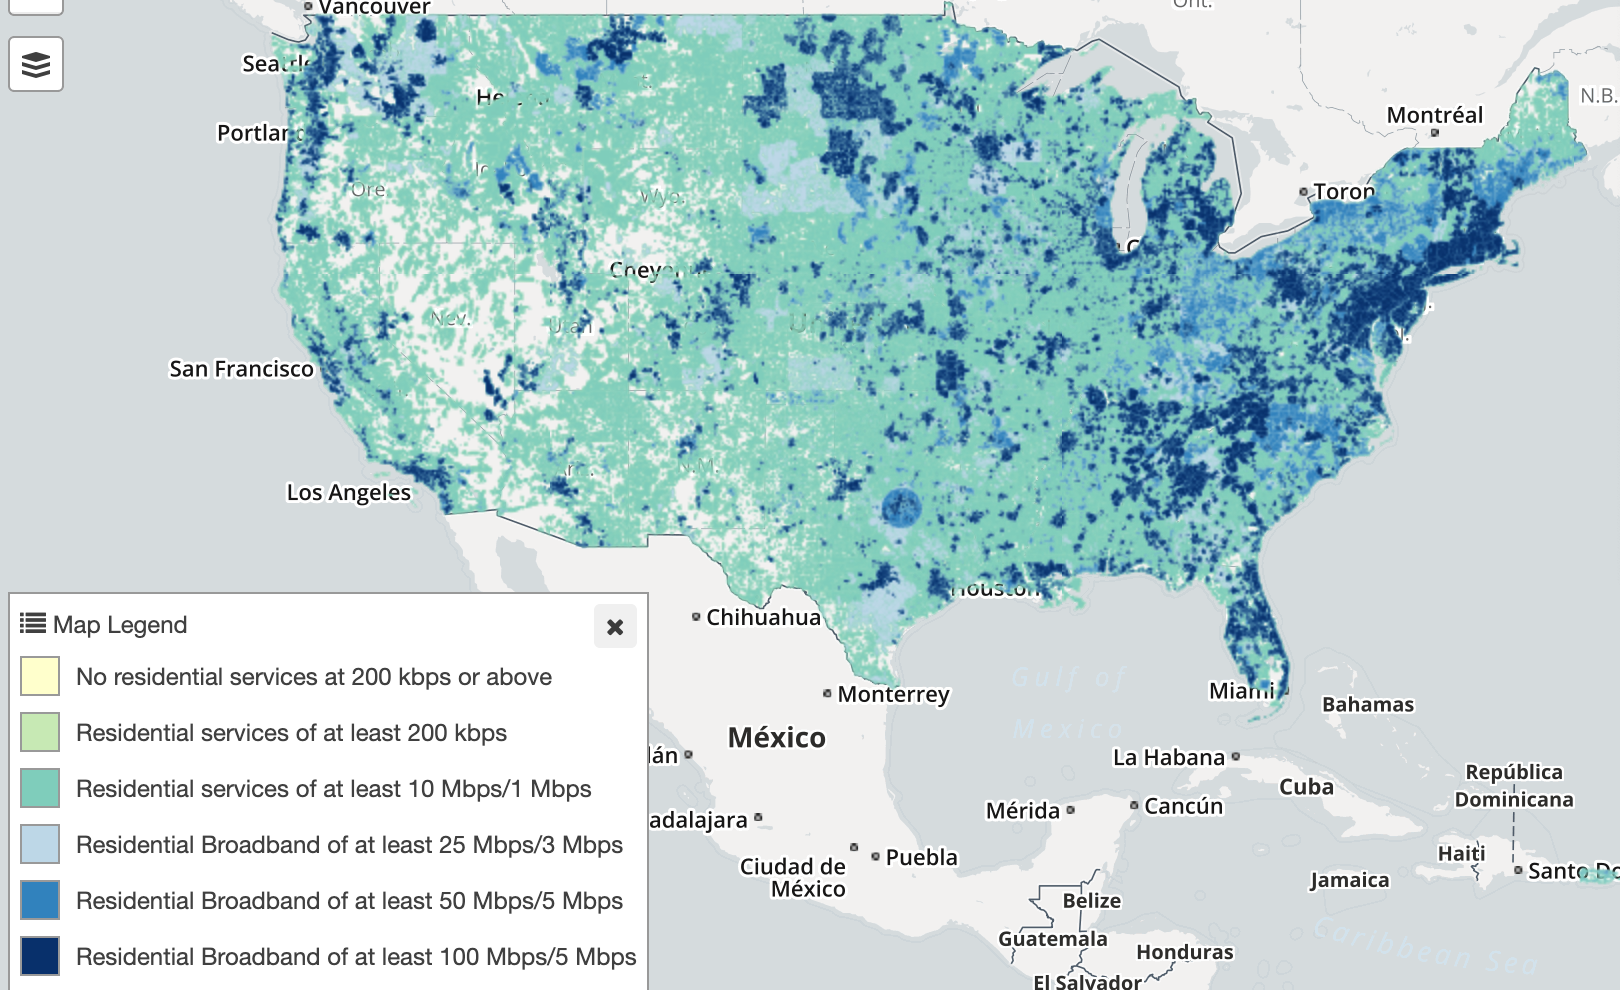
\includegraphics{images/other/FCC_Fixed_Broadmand_map.png}
    \caption{Maximum available connection speed across the \us}
    \label{fig:broadband_map}
\end{figure}

\subsection{Data Collection via the Postal Service}
One data source we considered was to utilize the \usps to send a small cellular connected device such as a phone around the \us via ground shipping. As it traveled it would continuously run traceroutes to many other \ip addresses that are located across the \us. This would give us data along the route there and back. Unfortunately, it is not possible to send a package somewhere and then get it back easily without someone to receive it on the other end. However, assuming this problem could be solved it would be a viable method.

% \subsection{Backbone Analysis}
% Backbone analysis was a proposed method for analyzing \caida \& \ripe Atlas traceroute data. Since traceroutes contain a complete list of all servers along a route, it would be possible to create a massive graph of the internet using all \ip address pairs known to be directly connected. From there it would be theoretically possible to identify routers that form part of the internet backbone based on frequency of occurrence, and to analyze the connectivity to \textit{those} instead. The reasoning behind this is that your \textit{average} internet connectivity is likely influenced much more by your ability to connect to the backbone than your ability to connect to arbitrary devices on the internet.

% However, \caida and \ripe Atlas data processing continued and the amount of unique \ip address pairs grew, it became clear that such an analysis would be infeasible. As discussed in \cref{sec:caida_results} the amount of unique \ip address pairs is in excess of 200 million, precluding any realistic graph-based analysis of the data in our timeframe with the hardware most immediately available to us.
